\chapter{Implementation Part -- Pipeline}\label{ch:impl_pipeline}

The objective of the thesis is to design and build a reliable, high-throughput streaming data processing pipeline for image processing, specifically embedding computation. The pipeline is intended to be used as an internal subsystem of the Recombee infrastructure, enabling businesses to offer new products. The system must download raw images from the internet, process them, and store them in internal storage. After successful storage, the pipeline computes the image representation and outputs it as the result.

\section{Pipeline Solution Architecture}
To meet the requirements of a high-performance and scalable stream pipeline, the pipeline relies on a Kafka message broker. The broker serves as a task queue (input) for the pipeline and its jobs and as a communication layer between pipeline stages. Kafka is designed to handle massive throughput and offers low-latency data feeds, which are essential for building a streaming pipeline that must maintain high throughput while providing low latency. Due to its distributed architecture, it provides concurrent access without blocking, enabling the pipeline to scale horizontally during peak requests. Kafka persists events on disk and replicates them across a cluster of brokers. This ensures that processing tasks remain durable and available even in the case of hardware failure. Kafka was chosen as the backbone of the pipeline because it serves as the interface through which the Recombee infrastructure communicates with other services, enabling easy integration with existing systems. Any other message queue that meets the specified criteria (scalability, durability, concurrent access) could be used in the pipeline.  

The pipeline itself follows a distributed, modular architecture. By decomposing the end-to-end process into discrete logical units (jobs), the system can independently scale computationally intensive tasks and provide clear checkpoints for failure recovery. This modularity ensures that a bottleneck in image downloading does not stall the embedding computation, and vice versa.

The implementation is structured into two primary components (Downloader and Embedder) that communicate via similarly named Kafka topics. The pipeline also uses an Image Reactor component to log and maintain the entire index of available images.

\subsubsection{Downloader}
The Downloader is a concurrent application written in Go that connects external data sources with internal storage. To ensure high availability and horizontal scalability, the service is partitioned into two decoupled layers: the Ingestion Layer and the Worker Pool.

\paragraph{Ingestion and Rebalancing} \mbox{} \\
The first layer manages a Kafka consumer that fetches tasks from the downloader topic and forwards them into the internal (Go channel) queue. By decoupling message ingestion from the actual download process, the service can perform online autoscaling and immediate consumer rebalancing. This ensures that even during heavy I/O operations, the service remains responsive to Kafka’s protocol, allowing for seamless distribution of the workload across new instances.

\paragraph{Concurrent Worker Pool} \mbox{} \\
The second layer consists of a pool of independent workers that process images from the internal queue. Each worker performs the following operations:
\begin{itemize}
    \item \textbf{Downloading:} Downloads an image from the internet to memory.
    \item \textbf{Metadata extraction:} Extracts metadata of the image (size, format, hash) from the image.
    \item \textbf{Storage:} Uploads the image to internal image storage and separated metadata storage (Image Reactor -- see below).
    \item \textbf{Notification:} After all successful operations, the job is published in the embedding topic to trigger the embedding computation.
\end{itemize}

Any failure during image processing is reported to the Image Reactor. By centrally logging these errors, the system enables subsequent examination and manual or automated retries. This reporting mechanism ensures that individual task failures do not stall the pipeline, allowing workers to remain highly available for subsequent tasks.

\subsubsection{Image Reactor}
The Image Reactor is an application that stores application metadata of downloaded images. It is a Python REST API designed to decouple physical storage locations from application-specific metadata. By acting as a specialized catalog, it provides the abstraction layer necessary to satisfy business requirements without placing additional load on the primary image storage system. Decoupling application and storage metadata is a concept proposed by the Haystack paper \cite{brewer_cap_2012}. While raw image data reside in a dedicated image store, the Reactor tracks associated attributes, such as resolution, format, and business-specific tags, that are essential for product usage.

The Reactor persists metadata in a dedicated and replicated PostgreSQL database, providing transactional guarantees for every record. The application is designed to be stateless, enabling horizontal scalability and high availability. The implementation employs a concurrency pattern to maximize throughput while keeping resource requirements, such as CPU and memory, low.

The Reactor also records all errors that occur during the data processing pipeline. It can be understood as a central logging system for pipeline failures. When a worker experiences any failure while processing the image, the Reactor records this failure. By logging these errors centrally, the system provides a clear mechanism for evaluating failed jobs and triggering manual or automated retries based on specific business logic. This ensures that individual task failures are isolated and do not stall the high-throughput processing of the remaining queue.

\subsubsection{Embedder}
The Embedder is the final component in the data processing pipeline. The application transforms raw image data into the corresponding embedding vector representation. Its architecture is similar to the Downloader: it consumes tasks from a dedicated Kafka topic. The Kafka message includes the image path in the internal image storage, along with the data required for correct image transformation. Similar to the Downloader, the Embedder can run multiple computations in parallel if needed. The ability to consume messages from Kafka and images from internal data storage simultaneously makes the Embedder horizontally scalable.  

\section{Pipeline}
The complete pipeline is a distributed system comprising multiple specialized components, including the Downloader, the Embedder, and the Image Reactor. Each component serves a strictly defined purpose within the data processing lifecycle, enabling the system to be precisely tuned to specific requirements. By decoupling these stages via Kafka topics, the pipeline enables scaling based on the required workload, a key objective of any streaming pipeline. For a complete overview of the system architecture and the data flow between these components, refer to the diagram in Figure \ref{fig:dt-pipeline}.

\begin{figure}[h!t]
    \centering
    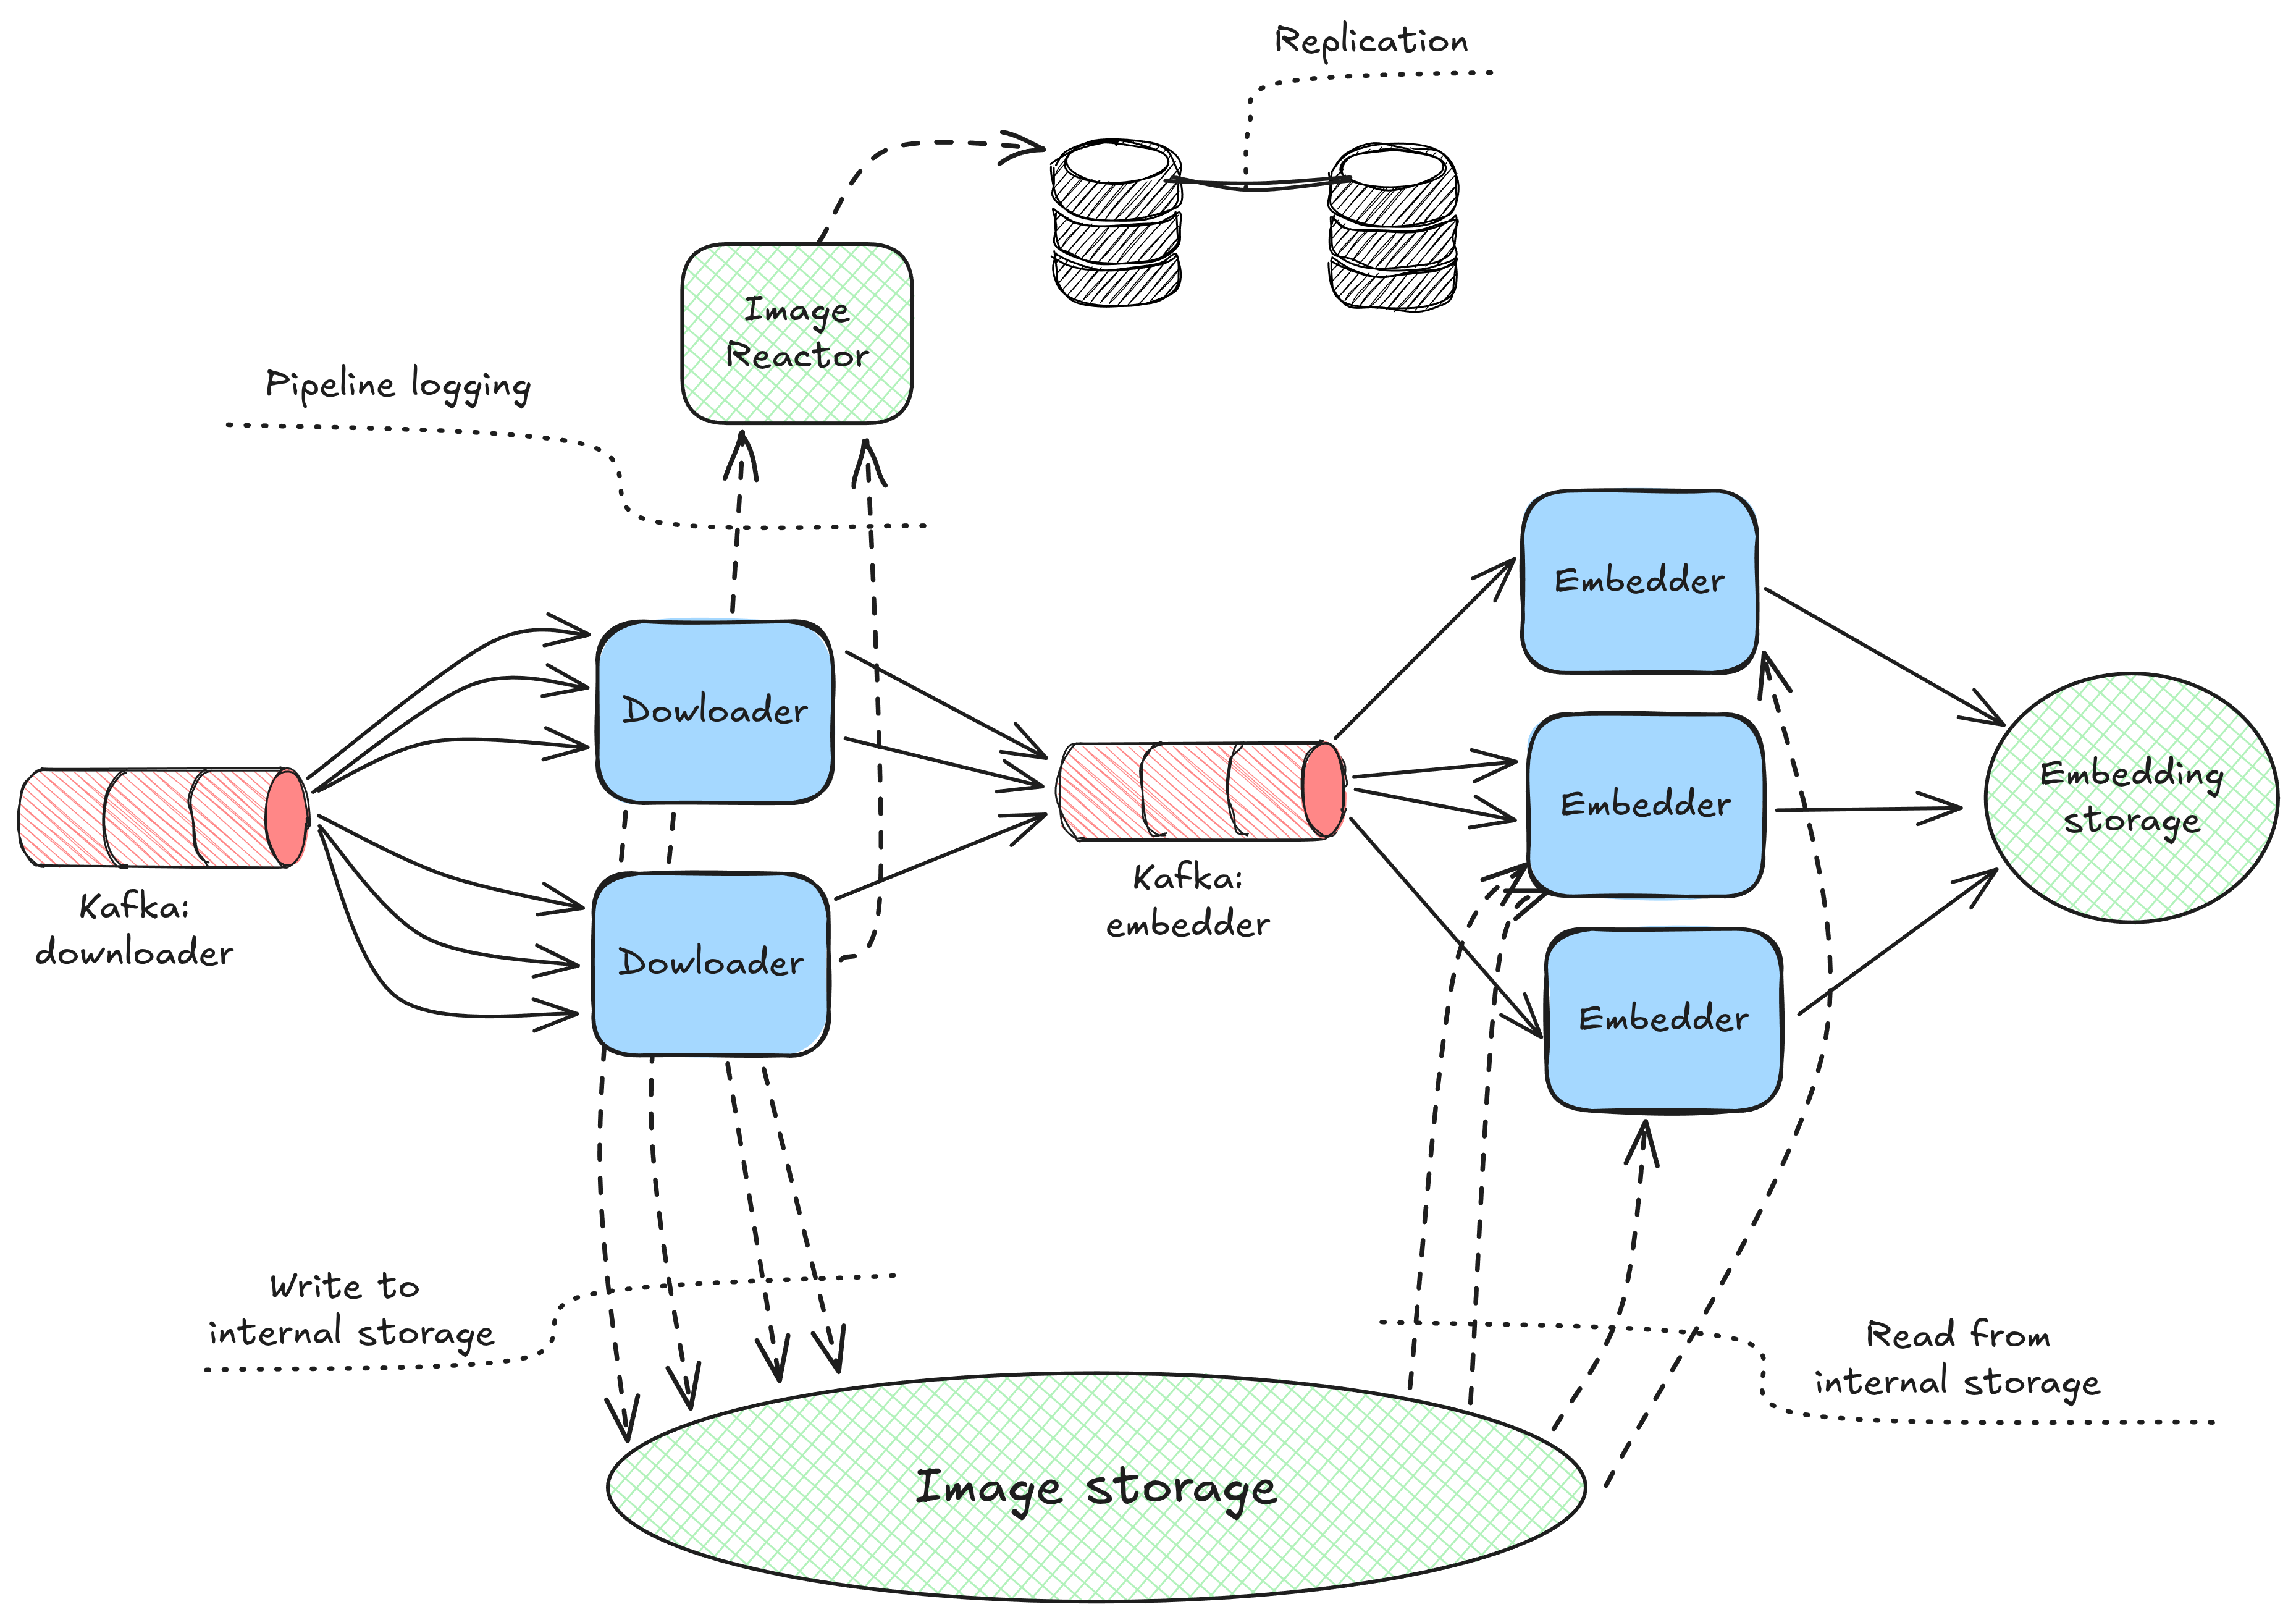
\includegraphics[width=0.9\textwidth]{images/dt-pipeline.png}
    \caption{\label{fig:dt-pipeline}Data processing pipeline architecture}
\end{figure}

\section{Deployment and Orchestration}
The components and pipeline described in the previous sections constitute the system's logical architecture. However, for the pipeline to function within a production environment, the setup must guarantee High Availability (HA) and scalability. Such properties can only be achieved by deploying the system across multiple nodes, with operations distributed across them.

There are several ways to achieve this orchestration over multiple nodes. For pipeline deployment, Kubernetes was chosen. Kubernetes is a container orchestrator that provides a way (almost standardized \cite{pope_why_2019}) to deploy applications. In addition to deployment, it is designed to handle service discovery, scheduling, networking, storage, and other required services. This makes it suitable for deploying the designed pipeline.

The Kubernetes orchestrator provides building blocks for building a pipeline that is HA, fault-tolerant, and supports scheduling and load balancing. To make the pipeline truly streamlined, automatic dynamic scheduling is needed for pipeline components. While automatic dynamic scheduling is not part of the core Kubernetes capabilities, it can be added through its extensible architecture. To enable automatic scalability, KEDA is used.

\subsection{Autoscaling}
KEDA (Kubernetes Event-Driven Autoscaling) is a component that extends Kubernetes to provide event-based scaling. KEDA enables the cluster to respond directly to external events and scale Kubernetes objects accordingly. It is designed to work natively with the Kubernetes API and can scale Deployments (stateless applications), StatefulSets (stateful applications), and Jobs (one-time tasks).

KEDA uses scaler plugins that provide event-based triggers. These scalers act as monitors of external services, such as databases and messaging queues. By monitoring these services, KEDA can trigger scaling actions based on the actual state of the data in these systems. One of those plugins is the Kafka Scaler. The Kafka Scaler enables autoscaling of Kubernetes components based on consumer lag. Kafka Scaler monitors the number of unread messages in a specific topic. If the lag increases, KEDA proactively schedules additional pods to handle a higher workload required to consume the Kafka topic. This ensures the pipeline is down-scheduled to minimal resources while remaining available in case no or low processing is required. On the other hand, when higher processing performance is required, KEDA can automatically horizontally scale the pipeline stages.

\vspace{1.5em}
The complete deployment example, including the code for each mentioned component, is provided in the attached media. 

\section{Properties of Pipeline}
The architecture of the designed pipeline, its deployment, and the implementation of its components meet the requirements of a streaming AI image-processing pipeline. The following list describes the implementation's specific technical properties.

\begin{itemize}
    \item \textbf{High Availability} \\
    All components in the pipeline, including Kafka and storage, are designed to offer high availability. The only component that does not fully support HA is PostgreSQL. Due to replication, it should be possible to switch to the replica if needed; however, this may result in partial data loss and a brief outage. Since the Image Reactor does not directly affect the pipeline, it should not affect the pipeline's availability.
    \item \textbf{Scalability and Throughput} \\
    The pipeline is designed to be horizontally scalable. Supportive storage may introduce limitations in scalability. PostgreSQL is designed to be vertically scalable rather than horizontally. To enable horizontal scalability of the Reactor's persistent layer, an alternative database technology should be considered. The Master server of SeaweedFS is the only component that is not horizontally scalable (for write) in the SeaweedFS deployment. During the design of the pipeline and the writing of the thesis, no evidence of its performance deficiencies was found. The last component that can influence scalability is Kafka. Kafka limits the number of consumers to the number of partitions used in the topic. It is a known limitation that is rarely encountered. To enable the pipeline to scale beyond the number of partitions in Kafka topics, a Consumer Proxy pattern can be used \cite{yang_enabling_2021}.
    \item \textbf{Monitoring} \\
    Because the streaming pipeline's internal processes are difficult to validate in production, all components expose metrics to enable visualization of the processes occurring within them. Pipeline components expose Prometheus metrics that are scraped by the Prometheus instance and displayed in the Grafana dashboard. The metric setup, including the Grafana dashboard, is included in the attached media.
\end{itemize}

The designed pipeline architecture and its specific implementation meet the requirements for high-throughput streaming AI image processing. During testing, no major problems were identified, and the system functioned as expected. The pipeline contains components that could limit its ability to scale horizontally, but these limitations are known and may be mitigated by the proposed improvements, in case such limits are met.